\section{NeurIPS 2025 Competition}
\label{sec:neurips}

Our \href{https://pokeagent.github.io}{NeurIPS competition} provided an opportunity to grow the research community’s interest in Pokémon and validate our evaluation protocols. Participants competed for prizes across both our Battling and Speedrunning leaderboards. The competition, which ran from July to December 2025, grew an online community of 650+ members and generated 150+ submissions. Here, we summarize the competition's results and key takeaways; additional rules and details can be found in Appendix \ref{sec:competition-retrospective}.


\subsection{Battling Track Results}

Participants in the Battling Track submitted agents to our AI-focused Showdown leaderboard, where they competed against fellow entrants and organizer-hosted baselines. The PokéAgent Challenge offers substantial improvements over prior agents (Figure \ref{fig:track1_baselines}); several of the strongest new baselines were kept private until the competition's conclusion to ensure that reaching the top of the leaderboard would require significant technical contributions. Figure \ref{fig:neurips_track1_main_text} visualizes the final standings. The top 8 teams in both formats qualified for a head-to-head tournament bracket, where both \#1 seeds (\texttt{PA-Agent} in Gen 1 OU, \texttt{FoulPlay} in Gen 9 OU) were eventually victorious. Members of the winning and runner-up teams provide details of their final solutions in Appendix \ref{sec:participant-methodologies}. Of the 16 qualifying spots, 13 were secured by teams extending our public RL baselines, while the remaining three were won by \texttt{Porygon2AI} (\#8 in Gen 9 OU) and \texttt{FoulPlay} \cite{FoulPlay} (\#1 in Gen 9 OU, \#8 in Gen 1 OU)---independent RL and search approaches, respectively. Appendix \ref{sec:track1-full-results} provides further analysis of the results, including the final tournament, and a comparison of alternative rating schemes.

\vspace{-2mm}

\begin{figure}[h!]
    \centering
    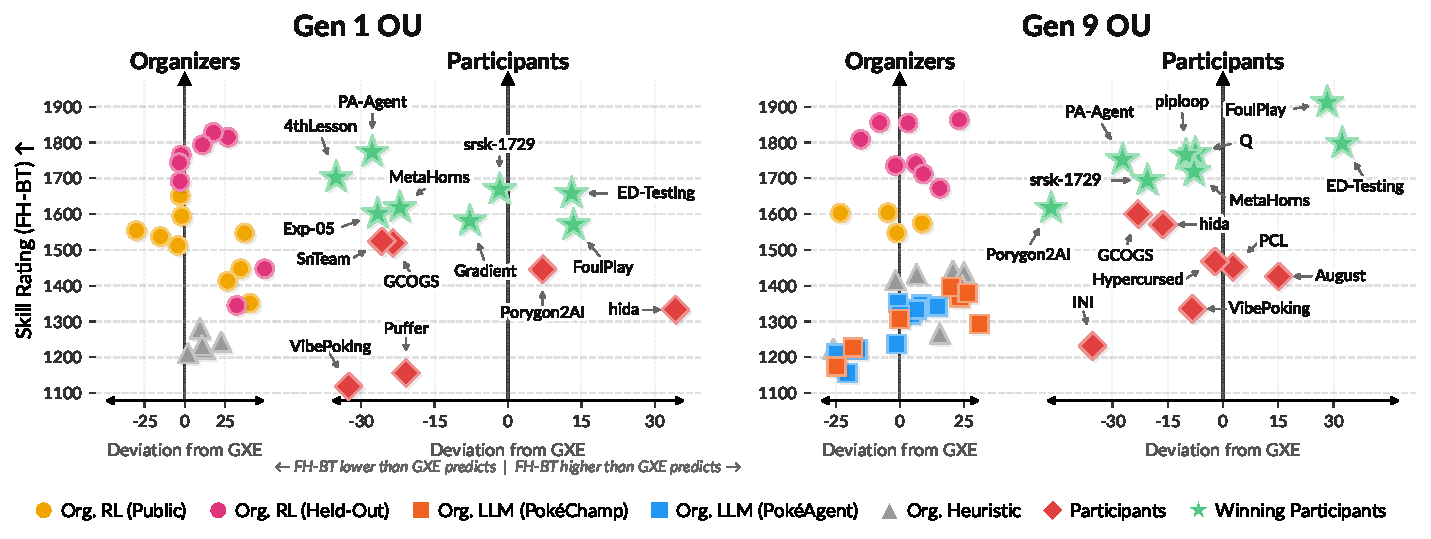
\includegraphics[width=\linewidth]{figures/track1_qualifying_strip.pdf}
    \vspace{-5mm}
    \caption{\textbf{NeurIPS Battling Leaderboard.} Organizer and Participant agent ratings are directly comparable. The x-axis measures disagreement between our primary rating metric and the linear trend established by GXE (a metric widely used on Showdown).}
    \label{fig:neurips_track1_main_text}
\end{figure}

\subsection{Speedrunning Track Results}

Of the 22 teams with valid submissions that submitted to the Speedrunning Track, 6 achieved 100\% completion (all 15 milestones). Figure~\ref{fig:track2_time_main} visualizes the final standings; full methodology descriptions appear in Appendix~\ref{sec:participant-methodologies}. The winner, Heatz, used Scripted Policy Distillation (SPD): an LLM decomposes the task into subgoals and generates scripted policies for each, which are then distilled into neural networks via imitation learning and refined with RL. The resulting agent completed the route in 40:13---nearly twice as fast as the second-place Hamburg PokéRunners, who used a pure RL approach (recurrent PPO with milestone-conditioned rewards). The remaining completions used LLM harness architectures with varying tool integrations (see Appendix~\ref{sec:track2-full-results}).

\begin{figure}[htb]
\centering
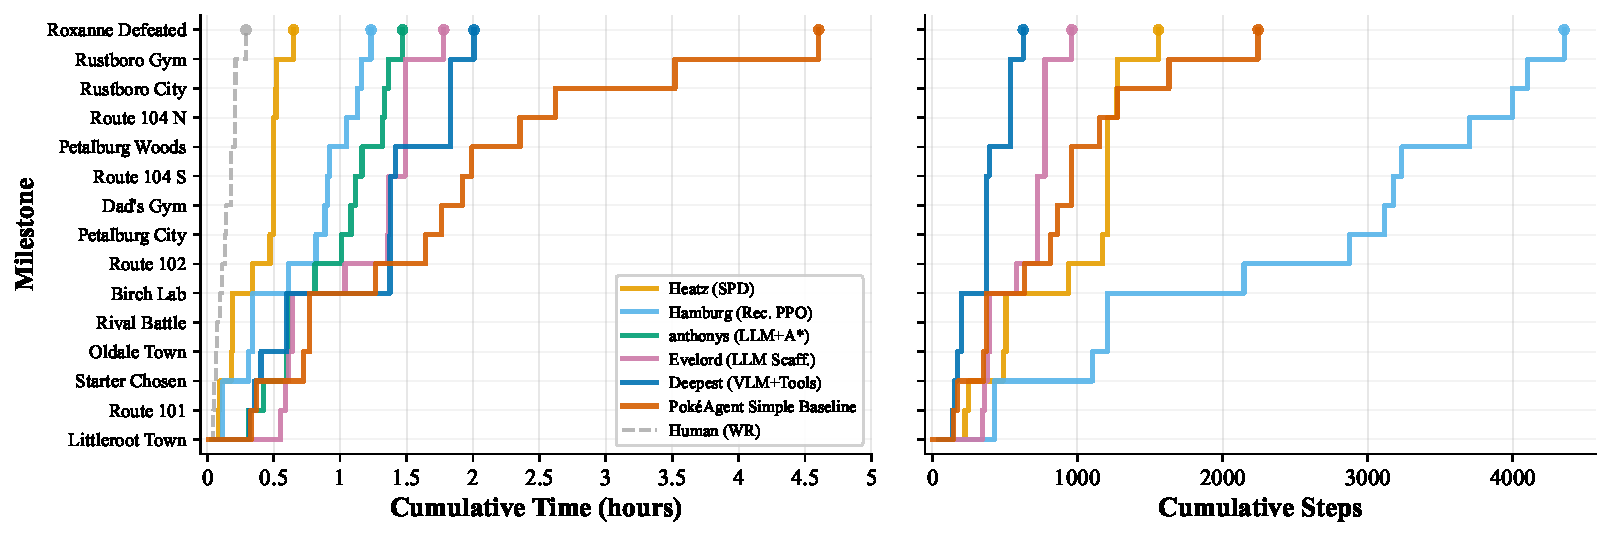
\includegraphics[width=\linewidth]{figures/track2_progress_time.pdf}
\vspace{-5mm}
\caption{\textbf{NeurIPS Speedrunning Leaderboard.} Milestone progress vs.\ wall-clock time (left) and cumulative agent steps (right) for the six teams that completed all 15 milestones. Unlike most game benchmarks that pause between actions, our environment runs in real time---the game world continues while the agent reasons, making inference latency a first-class cost. We therefore report both wall-clock time (end-to-end throughput) and step count (sample efficiency). This distinction reveals that Deepest$^\dagger$ (Judge's Choice) completed in the fewest steps (649) despite ranking 5th by time, highlighting the tradeoff between inference speed and action efficiency.}
\label{fig:track2_time_main}
\end{figure}



Time-based rankings do not tell the full story. When measured by total actions rather than wall-clock time, Deepest---5th by time---completed with the fewest steps (649 vs.\ Heatz's 1,608), pointing to a tradeoff between inference speed and sample efficiency. Heatz's RL-distilled policy executes far faster per step, compensating for the higher step count.

Without a harness, raw frontier VLMs achieve effectively 0\% task completion on this track. Pokémon Emerald gameplay is out-of-distribution for these models, and raw model calls produce agents that wander aimlessly, repeat failed actions, or become stuck in dialogue loops. A harness---perception, memory, planning, and action modules---is not a marginal optimization but a prerequisite for any progress. Furthermore, not all harnesses are equal: common CLI-agent architectures (e.g., Claude Code, Codex CLI, Gemini CLI) fail to maintain coherence over the thousands of sequential decisions required, despite using the same underlying frontier models that succeed with our domain-specific harness (Figure~\ref{fig:track2_results}). Long-context autonomous embodied tasks appear to demand qualitatively different architectures than single-session coding workflows. Particularly, in the effective use of robust long-term memory abstractions coupled with detailed and consistently iterated plans specified at sufficient levels of granularity. Absent of the effective employment of these abstractions, we find that CLI-agent architecures frequently make erroneous assumptions about their game progress and struggle to effectively localize their game progress within the broader contunity of milestone objectives in Pokémon Emerald. This gap likely extends to other OOD embodied domains requiring very long-context coherence.

\subsection{Cross-Track Insights}

\paragraph{Specialist methods outperform generalist LLMs.} Both tracks show a consistent pattern: RL and search methods outperform LLM approaches. In battling, the top participants all used RL or MCTS rather than LLM reasoning. In speedrunning, the top two finishers used RL-based methods. Heatz's 40:13 is more than $2\times$ faster than the best pure LLM harness approach (anthonys, 01:29:17). Put differently, Pokémon tasks require precise computation---probability estimation, opponent modeling, spatial planning---that current LLMs do not reliably perform from prompts alone.

\paragraph{LLMs as priors, RL as refinement.} Despite this gap, LLMs played a key role in the winning speedrunning approach. Heatz used an LLM to decompose the task and generate initial scripted policies, then distilled these into neural networks via RL. The LLM provided the prior (task structure and initial behavior) while RL provided refinement (faster execution and strategy discovery). This pattern---using LLMs for high-level reasoning and RL for low-level optimization---seems applicable beyond games.

\paragraph{Pokémon exposes reasoning failures that standard benchmarks miss.} In battles, weaker models exhibit ``panic behavior'' (also observed by \citep{gemini2p5report}): after a small tactical error, they compound mistakes rather than recovering, losing games they could still have won. Different model families fail in distinct ways---memory corruption cascades, goal oscillation, excessive plan commitment, and computational paralysis (see Appendix~\ref{sec:extended-discussion} and Figure~\ref{fig:cot_visualization}). These failure modes do not appear in coding or math benchmarks, where questions are independent. Pokémon's multi-turn, adversarial setting tests whether models recover from mistakes under pressure.

\paragraph{Pokémon battling is orthogonal to standard LLM benchmarks.} BenchPress~\citep{papailiopoulos2026benchpress} shows that an 83-model $\times$ 49-benchmark evaluation matrix is approximately rank-2: two latent dimensions explain $>$90\% of score variance, and 5 benchmarks suffice to predict the remaining 44 within $\sim$7 points. We added our Battling Track GXE scores for the 16 models that overlap with BenchPress. Pokémon breaks this low-rank structure: no existing benchmark correlates strongly with GXE (max Spearman $\rho = 0.77$; mean $|\rho| = 0.45$), and the rank-2 SVD that explains 91\% of standard benchmark variance captures only 27\% of GXE variance. Several models that score at frontier level on standard benchmarks collapse in battles, and vice versa. Competitive Pokémon appears to measure capabilities---strategic reasoning under partial observability and adversarial pressure---that are nearly orthogonal to what current evaluation suites capture.